

\chapter{Isle Royale: A Modeling Example}

\begin{marginfigure}
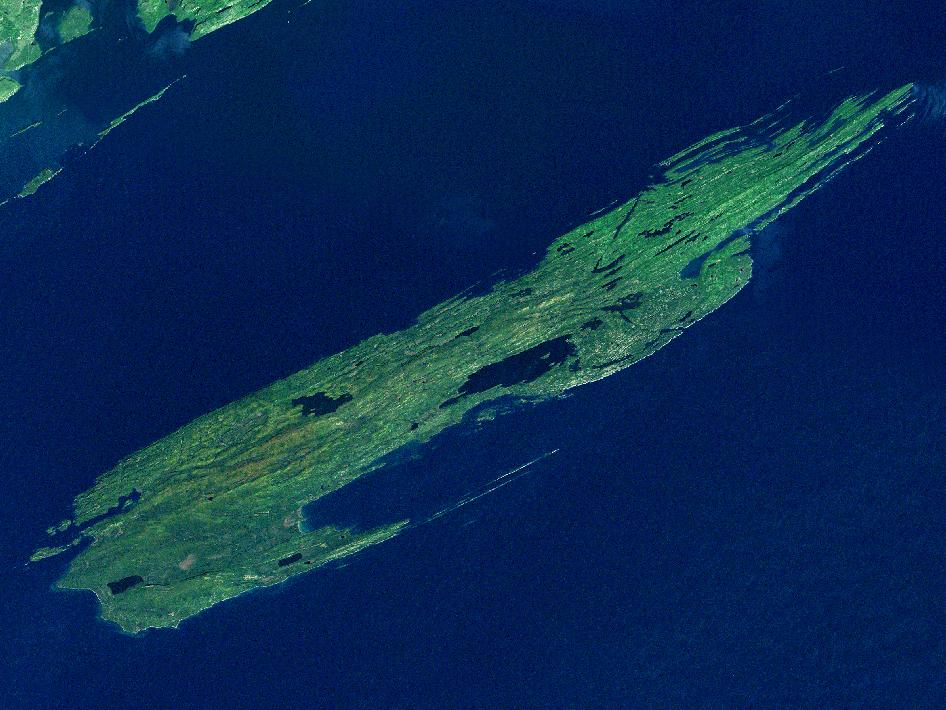
\includegraphics[width=5cm]{figs/IsleRoyale}
Image from {\em{http://finickymeterisnotavailable.blogspot.com}}
\end{marginfigure}


\section{A Biologist's Dream}
Isle Royale is a large island (about 45 miles long and 9 miles wide) in northern Lake Michigan.  The island and surrounding waters are a national park.  It's a pretty isolated place -- miles from the mainland, largely uninhabited, bitterly cold in the winter.

Perhaps the greatest claim to fame for Isle Royale is its population of wolves and moose.   According to the Michigan Tech's Wolf-Moose project, The first moose arrived on Isle Royale (presumably by swimming) in the early 20th century.  They were followed in the 1940s by a population of wolves, which got to the island by crossing an ice bridge from Canada.  Such ice bridges are rare occurrences, so effectively, the wolves and moose have been ``locked'' on Isle Royale for the last 70 years.

Of course, wolves eat moose, and in the context of the island, the moose turn out to be the major food source for the wolves.  At the same time, the moose on the island don't really face any other predators besides the wolves.  Thus, the island (theoretically, at least) provides an ideal, naturally-occurring, experiment in the dynamics of a predator-prey system.  Such a naturally occuring, isolated system is pretty darn rare, and so biologists and ecologists have followed wolf and moose populations on the island since the mid 50's.

In this case study, we're going to look at the Wolf-Moose system on Isle Royale.  We'll try to abstract a model for this system; we'll use the model to make some predictions; we'll try to validate our model; and ultimately we'll refine the model to the point where we might (or might not) be able to do some useful work with it.  So let's get started.

\section{Where to begin?}
To start with, we could take a couple of routes.  

One option would be to just start making assumptions, doing back-of-the-envelope calculations, etc.  In doing this we would almost certainly end up ``re-inventing the wheel''.  We would also make mistakes that others have made previously, and we'd probably end up with a model that is not as accurate as existing models.  On the other hand, we'd probably learn a lot in the process.    And, as we progressed, we'd probably end up looking things up -- so our research would be targeted, instead of scattershot.  

The other option, of course, is to spend some time to delve into the existing research about Isle Royale.  This would not be a bad thing to do in this particular case -- after all, it is a system that has been studied to death.  Of course, we'd run the risk of discovering that there are many existing models for the populations on the island.  We might also find that those models are quite a bit more complex than the kind of model we're going to build.  So we'd be very well-informed, but we'd also feel sad, because we would feel we had nothing to contribute.  But the reality is that, in many situations, existing models have become sufficiently complicated that they are not necessarily useful.  Usually the best model for doing certain kinds of work is not the most complex model, but rather is the model that is only complex enough.  So even if we find out that there's a lot of existing work, that's not a reason to avoid the topic.

The reality in modeling and research is that you tend to bounce back and forth between these two approaches.  Starting without looking around a bit is foolish, but spending all your time looking around without actually trying stuff is foolish too.  So let's try to split the difference here.

\section{Background on Isle Royale}

As we predicted above, it's pretty darn easy to track down information on Isle Royale.  About 15 minutes on the internet yields an awful lot information: \sidenote{see {\tt wikipedia}, and {\tt isleroyalewolf.org}}
\begin{enumerate}
\item The average number of moose that a wolf kills per month is about 1 (with significant variation).
\item Ticks and disease load play a major role in the moose population.
\item The availability of balsam forage is important for the moose population, and there has been significant variation in balsam population due to moose foraging.
\item Historically, the wolves have suffered from lack of genetic variation.
\item The population of wolves averages around 23.
\item The wolves are divided into a small number of packs.
\item Wolves tend to kill sick or old moose.
\item Climatic effects are important -- heavy snows increase malnutrition in moose; mild winters lead to large tick and disease loads.
\item About 85\% of moose deaths can be attributed to wolves as the proximate cause.
\end{enumerate}

It also doesn't take long to find a LOT of data.  For example, {\tt http://isleroyalewolf.org}'s data page includes raw data about wolf and moose populations, as well as all kinds of other stuff (kill rates, moose age population structure, genetic diversity in the wolves, etc., etc., etc.).  And, as can be seen in Figure 1, the reality of wolf and moose populations on Isle Royale is a bit messy -- sharp peaks, significant year-to-year variations, etc.

\begin{figure}
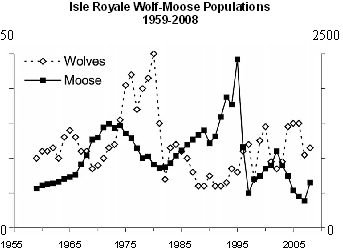
\includegraphics[width=4in]{figs/wolfmoosedata.jpg}
\caption{Wolf and moose populations on Isle Royale, from {\tt isleroyalewolf.org}}
\end{figure}

\section{As Simple as Possible}

At this point, we have a ton of information -- and that information is more than a little daunting.  After all, it sounds like a model for this system ought to include ticks, balsam fir, weather, genetics, wolf social behavior, moose disease.  Ugh!

The key to moving ahead here, and to moving ahead in modeling generally, is to {\em start simple}.  Try to identify the stuff that matters most of all, work with that, and then -- once you understand the simplest model possible, ask two questions:
\begin{enumerate}
\item What work can you do with this model?
\item What is the next step to take in improving the model?
\end{enumerate}

For the case of Isle Royale, if we really wanted to start simple, we would {\it probably} focus just on the moose-wolf interaction.  We'd ignore ticks; we'd ignore weather; we'd ignore variations in balsam population; we'd ignore genetics; we'd ignore age structure in the populations, and so on.  In other words, we'd abstract away a lot of the detail in order to build a simple model.

\subsection{Simple Qualitative}
So what does this simple model look like?  Well, the simplest thing might be to just start with the moose, and identify the different processes by which the number of moose change.  There are at least three we can think of easily:  moose are born, moose die of natural causes, and moose die through the action of wolves.  A qualitative stock-and-flow that captures these ideas about the moose might look like this:

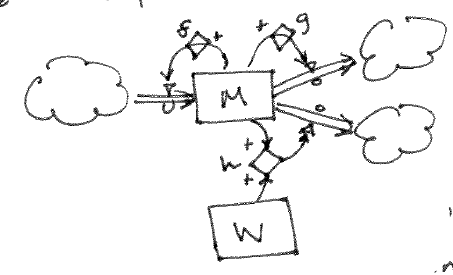
\includegraphics[width=8cm]{figs/QualitativeMooseStockAndFlow}

If we translate this directly to a difference equation, we get a very qualitative difference equation:
$$M(t+1) = M(t) + f(M(t)) - g(M(t)) - h(M(t),W(t))$$
where $f(M)$ is some function that tells you the number of moose births given the population of moose, $g(M)$ tells you the number of natural deaths given the current moose population, and $h(M,W)$ tells you how many moose die at the paws (jaws?) of wolves, for a given moose and wolf population.

It's also easy to imagine an analogous stock and flow for wolves, which would give a difference equation that looked like this:
$$W(t+1) = W(t) + a(W(t)) - b(W(t)) - c(M(t), W(t))$$
where $a(W)$ is the number of wolf cubs born, given the current wolf population, $b(W)$ is the number of wolves that die due to causes other than starvation for a given wolf population, and $c(M,W)$ is the number of wolves that die from starvation, given the moose and wolf population.

\subsection{Simple Math}

At this point we have two difference equations that pretty undefined:  the functions $a(M)$, $b(M)$, $c(M,W)$, etc. are only specified to the extent that we can say that $c$ probably increases as both $M$ and $W$ increases, $a$ and $b$ both increase as $M$ increases, and so forth.  But any number of functions would do that.  How can we decide what the right function is?

As we've discussed already, keeping the model simple to start with is a good general principle: you can always increase complexity later.  In general, there are a number of ``keep it simple'' strategies that can help you to decide what function to use.  Here are some of them:
\begin{itemize}
\item {\em Use experimental data} to figure out what the function should be.  If you can look at the data and see pretty strong behavior, you can often decide on your function immediately.  For example, you could imagine that the data on Isle Royale might contain information about the number of moose calves each year.  If, in plotting that data, you found that  the number of moose born each year was proportional to the number of moose), you'd be pretty well justified in claiming that $f(M)$ is proportional to $M$.
\item {\em Use common sense} to decide on your function.  In general, if you have more mother and father moose, you'll have more baby moose.  It's not hard to make the physical argument that, at least under some circumstances, $f(M)$ ought to be proportional to $M$, because ``that's how reproduction works''.   Naturally this argument doesn't hold in all cases, but since we're keeping things simple, it's a pretty reasonable argument to make.
\item {\em Use mathematical simplicity} to decide on your function.  For moose births, you need a function $f(M)$ that increases as $M$ increases.  Although there are an infinite number of possible functions, the simplest one is setting $f(M)$ to be proportional to $M$.
\item {\em Limit your model to a particular regime.}  For example, in the limit of very small moose populations, it seems obvious that the number of births each year might vary from year to year, depending on how successful individual moose were in finding mates.  By the same token, at very high population densities, it's possible that the moose would reduce their reproduction rate due to lack of food.  


\end{itemize}
think about two stocks:  wolves, and moose.  Wolves are born and they die; moose are born and they die, and the two species interact in these processes:

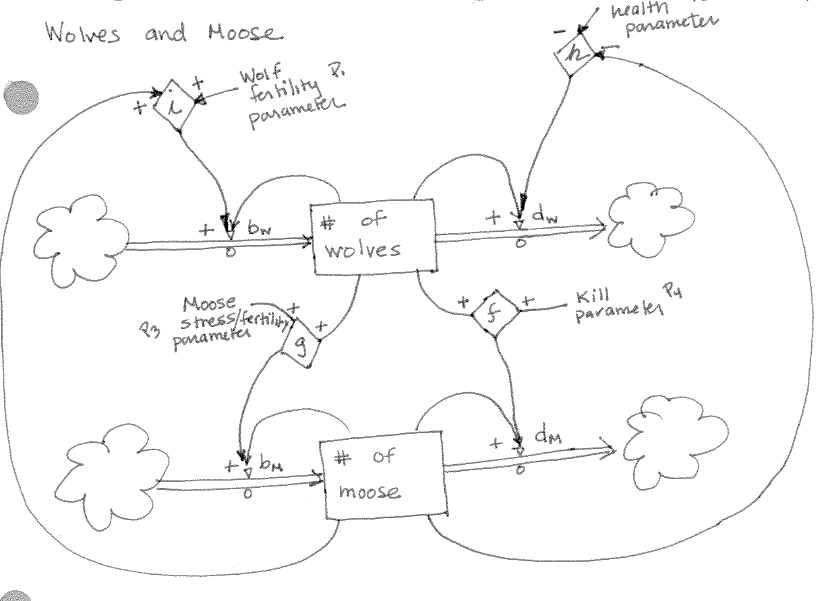
\includegraphics[width=12cm]{figs/WolfMooseStockAndFlow}

At first blush, we might expect that the birth and death rates for both species will depend on the populations of both species.  For example, presumably increasing the number of wolves will result in a greater wolf birth and death rate; it will also probably result in an increased moose death rate, and (perhaps) a decreased moose birth rate (due to increased stress).  Similarly, increasing the moose population might increase the wolf birth rate (``yay, more food -- let's make more baby wolves!'') and reduce the wolf death rate (``I was going to die, but now there's more moose for me to eat...'') as well as increasing both birth and death rates for moose.

It's worth noting that this model is only going to be able to answer a limited set of questions.  We could not, for example, use this model to explore the impact of ticks on the moose population --we chose to abstract ticks away.  We couldn't really explore climatic impacts either.  

Furthermore (and perhaps not as obviously), this model is probably not going to be terribly useful for making real numerical predictions.  Because we've simplified so far, it's unrealistic to expect that the model will actually tell us {\it numbers} that are terribly reliable.  Rather, it will be a better model for gaining qualitative insight.  So asking, ``How many wolves can Isle Royale sustain?'', while possible, is probably not very useful -- whereas asking ``What kinds of behaviors do we see for different wolf populations?'' might make more sense.

\section{Building the mathematical model}
Even though the stock-and-flow above {\it looks} pretty simple, it suggests a nastily complex set of difference equations:  we have two birth rates, and two death rates, each of which depend on both the wolf and the moose populations.   So its utility as a model representation is that it allows us to think about how these flows depend on different quantities -- but it may not be quite so useful for generating equations.


With the stock-and-flow representation in mind, we now want to construct a mathematical representation -- a set of difference equations.  To simplify matters, we will write the difference equations in terms of the net change in both populations, as opposed to making a distinction between changes due to deaths an changes due to births.  Taking this approach, a general version of the difference equations can be written as 
$$M(t+1) = M(t) + \Delta M(M(t), W(t))$$
$$W(t+1) = W(t) + \Delta W(M(t), W(t))$$
where $\Delta M$ and $\Delta W$ are functions that describe the yearly change in the moose and wolf populations implied by a particular level of moose and wolf population.

\subsection{Changes in moose population}
Now, with this formalism, we start to think about what the model might look like in more detail.  Let's try thinking about how $\Delta M$, the yearly change in the moose population, might depend both on the number of moose and wolves.  

Let's start by assuming that there are no wolves on the island at all. The stock and flow we drew suggests that the population of moose will just be first order (i.e., $\Delta M \propto M$).  We might take this a step further (thinking about those balsams), and imagine that $\Delta M$ might look like a simple carrying capacity model like we have seen previously:

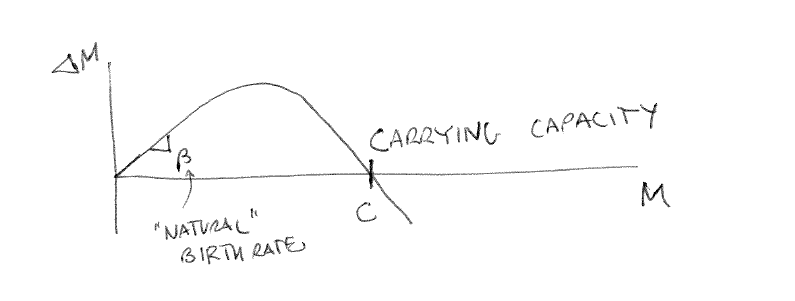
\includegraphics[width=12cm]{figs/DeltaMvsM}


Here we see that for small moose populations, $\Delta M$ is proportional to the population (i.e., twice as many parents make twice as many babies, and since the island has plenty of room, the population grows).  As the population rises, though, $\Delta M$ levels off, and finally drops to zero at the carrying capacity.  At this point reduced resource availability has made the death rate high enough to offset the birth rate.  Finally, if the initial moose population is greater than the carrying capacity, we see that $\Delta M$ is negative -- in other words, more moose are dying from starvation each year than are born into the population.

Thinking about how $\Delta M$ relates to $W$ is a bit harder.  Let's start by thinking about what the wolf population tells us.  Effectively, the more wolves there are, the greater the chances of a moose encountering a hungry wolf (or pack of wolves).  So, we expect that $\Delta M$ to drop as the wolf population increases.  At some critical wolf density, the chances of a moose having a baby are the same as the chances of the moose being eaten by a wolf or dying due to natural causes.  At this wolf population, $\Delta M$ is zero.  And, for  large wolf densities, $\Delta M$ is negative:  moose are more likely to be eaten or to die than to reproduce.


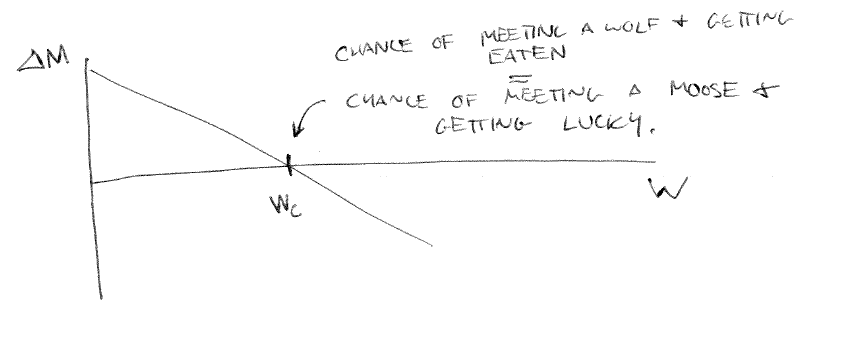
\includegraphics[width=12cm]{figs/DeltaMvsW}


Combining these two bits of analysis, it's not hard to imagine what $\Delta M$ might look like as a function of both of these quantities. Qualitatively, we expect something like this:


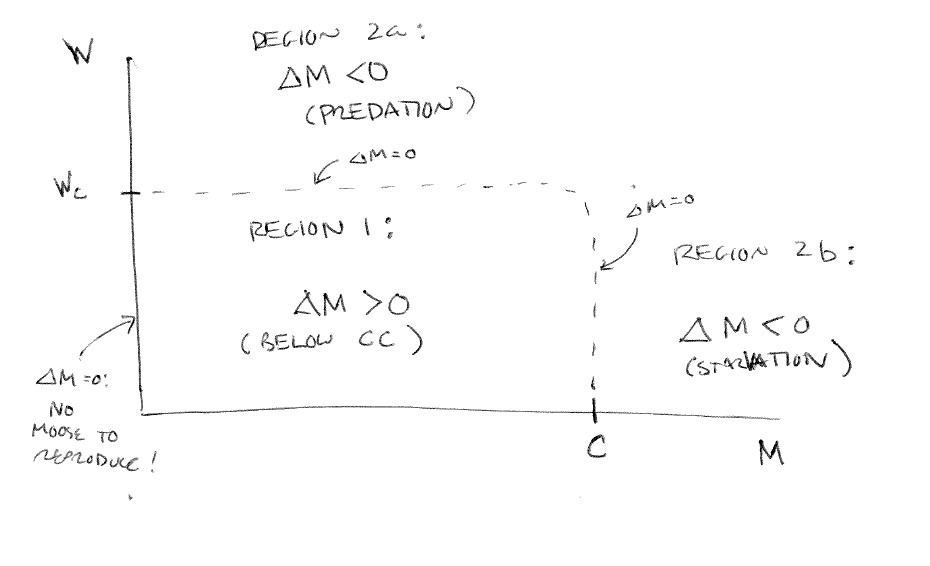
\includegraphics[width=12cm]{figs/DeltaMPhasePlane}


There are two regions here.  In region 1, the population of moose is below carrying capacity, and the density of wolves is low enough that moose are more likely to reproduce than to be eaten.  As a consequence, in this region, $\Delta M >0$ .  In region 2, either the density of wolves is high enough that moose are more likely to be eaten than to reproduce (2a), or the population of moose is above the carrying capacity, so (in both instances) $\Delta M<0$. 

Mathematically, we might try to capture this kind of behavior with the following expression:

$$\Delta M = \beta(1-\frac{M}{C})(1-\frac{W}{W_c})M$$

where $\beta$ is the ``natural'' net birth rate (in the absence of wolves and starvation), $C$ is the moose carrying capacity, and $W_c$ is the ``critical wolf density'' -- the density at which the chance of a moose getting lucky with another moose is identical to the chance of a moose running into a wolf.

\begin{del}
 It's worth thinking about units and numbers here:  what are the units of $\beta$?  Of $C$?  of $W_c$?
\end{del}

\begin{del}
It's also worth thinking a little harder about the mathematical model above.  We've made a pretty serious modeling mistake here -- what is it?  Where is the error?
\end{del}

Let's recall our plan to keep things simple:  we said we were ignoring everything that we possibly could.  Carrying capacity is interesting, but for now let's kill it, and just assume that moose populations are small enough that first order growth is sensible.  Then
$$\Delta M = \beta(1-\frac{W}{W_c})M$$
In this case, it is worth noting that the death due to wolf-moose interactions in this model is proportional to the product of the moose population and the wolf population -- i.e., it is proportional to the probability of  a wolf-moose interaction.  

\subsection{Changes in wolf population}
We can pursue a similar model for $\Delta W$.  Since wolves depend on moose for sustenance, there is some minimum moose population that supports the existence of wolves.  Below this moose population, $\Delta W <0$; above this moose population, wolves are happily eating moose to reproduce. 


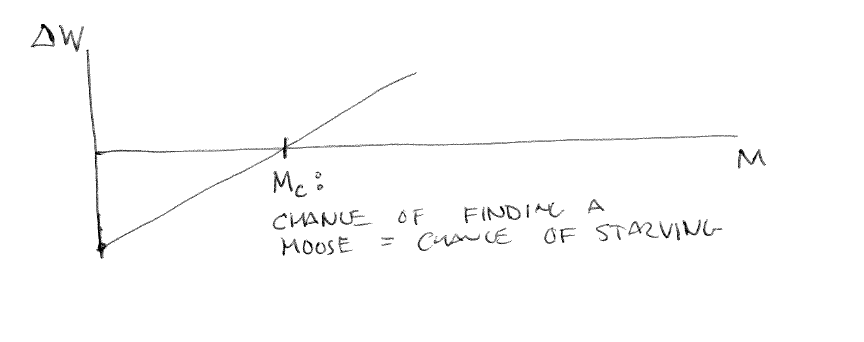
\includegraphics[width=12cm]{figs/DeltaWvsM}


Using a similar argument to the one we employed for the moose, we imagine what $\Delta W$ might look like as a function of both of W and M. Qualitatively, we expect something like this:


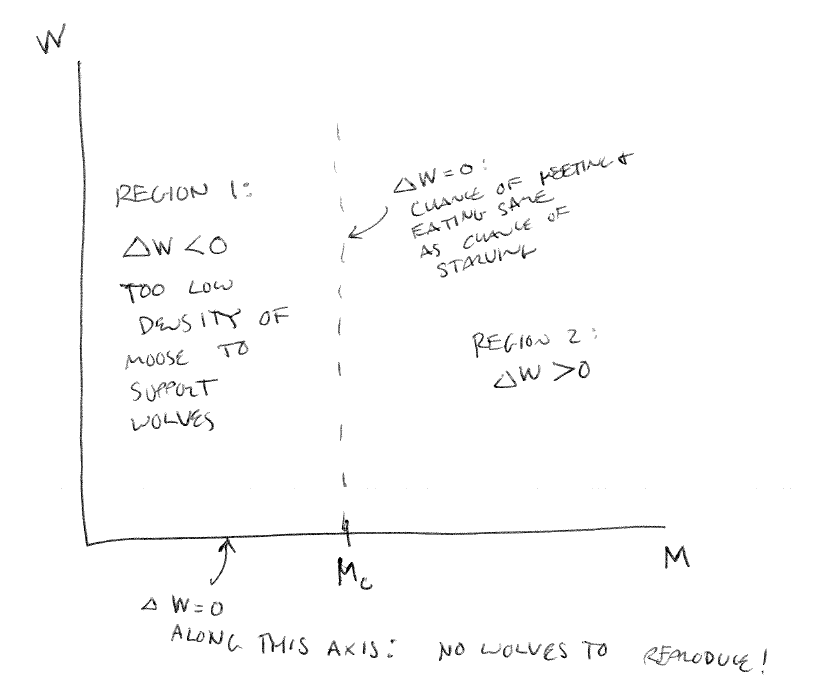
\includegraphics[width=12cm]{figs/DeltaWPhasePlane}

To the left of $M_c$, in region 1, the wolves are dying of starvation.  Naturally the number of deaths increases as the number of wolves increases (more wolves to die), and also increases as the number of moose decrease (more starvation).  In region 2, the number of wolves is increasing, because there is a high enough density of moose that wolves are more likely to encounter a moose than to starve.  Here, of course, higher wolf populations also lead to larger increases in wolf population -- more wolves to make wolf puppies!

Mathematically, this can be captured with the model
$$\Delta W = \gamma(\frac{M}{M_c}-1)W$$
where $\gamma$ is the natural net {\it death} rate of wolves in the absence of moose, and $M_c$ is the critical moose density required to support a wolf population.

\subsection{Haven't we seen this before?}

We've been arguing thus far for simple expressions for $\Delta M$ and $\Delta W$ -- and in the process, we have ended up (not surprisingly) with a re-statement of the Lotka-Volterra predator-prey model that we discussed in the previous chapter.   It might be worth going back and taking a look at this now:  you'll recall the following pictures (now modified by replacing rabbits with moose, etc.:

\beforefig
\centerline{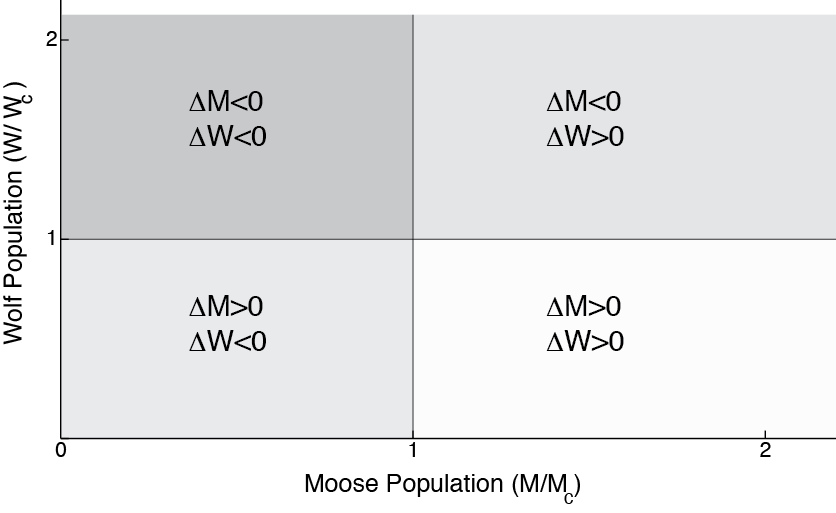
\includegraphics[width=8cm]{figs/WolfMoosePhasePlaneRegions}}
\afterfig

Starting in the lower left-hand corner, $M<M_c$, and $W<W_c$.  Consequently, wolves are dying ($\Delta W<0$), and moose are multiplying ($\Delta M>0$).  As $M$ increases, we reach a region where  $M>M_c$, and $W<W_c$.  This implies that there are now enough moose to support wolves, so $\Delta W>0$, while at the same time the number of wolves is too small to suppress increase in the moose population, so $\Delta M>0$.  Similar analysis applies to the remaining regions, giving us the following (qualitative) phase plane plot:

\beforefig
\centerline{
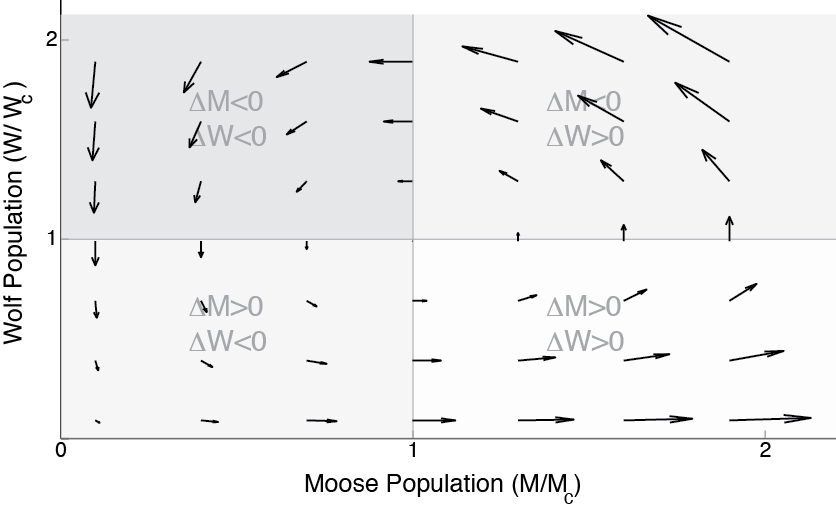
\includegraphics[width=8cm]{figs/WolfMoosePhasePlaneQuiver.png}}
\afterfig


 \section{Choosing parameters}
 
Now that we have a first pass at the mathematical model, we'd like to be able to implement this (either in MATLAB or by hand) in order to actually see how this model behaves in comparison to the actual physical system.  To do so, we clearly need to choose some parameters:  what {\it numbers} (with {\it units}) will we use for $M_c$, $W_c$, $\beta$, and $\gamma$?

\subsection{Finding $M_c$ and $W_c$}
Well, examination of the data gives us a good first cut at some of these values.  Let's look at it again:

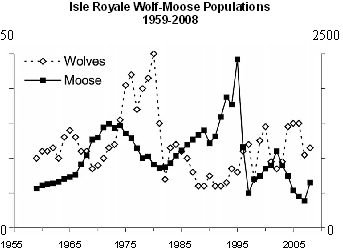
\includegraphics[width=4in]{figs/wolfmoosedata.jpg}
 
 It appears that the wolf populations varies around a typical value of about 25.  So it's not unreasonable to choose (as a first guess) $W_c = 25$ wolves.  Similarly, moose populations seem to oscillate around a baseline of around 1000.  So let's choose $M_c = 1000$ moose.  Why did we make these choices?  Well, the phase plane plot shows that the populations ``circle around'' the equilibrium values of $(M_c,W_c)$ -- so we're choosing values that $M$ and $W$ seem to be ``circling around''.

\subsection{Net birth and death rates}
From our research, we know that each wolf kills about one moose per month -- and we know that most moose are killed by wolves.  Looking at the expression for $\Delta M$, 

$$\Delta M = \beta(1-\frac{W}{W_c})M$$

we see that the kill rate $K$ (the number of moose killed per wolf per time step) is 

$$K = \frac{\Delta M_{killed}}{W} = \beta \frac{M}{W_c}$$

If we assume that $M=M_c$, find that  $ \beta = K \frac{W_c}{M_c}$ moose per moose per month.  Since $W_c = 25$ and $M_c = 1000$, we obtain $\beta = .025$ (for a time step of one month). 

Let's think about whether that value makes sense.  This value says that, in the absence of wolves, the net growth rate for moose is .025 moose per moose per month.  This implies a doubling time of about 28 months.   Looking back at the data, this doesn't seem insane -- there are certainly periods in which the population grows almost this quickly, but there don't appear to be any periods in which it's faster than this.

Finally, let's think about $\gamma$.  $\gamma$ tells us what the death rate is of wolves in the absence of moose:
$$\Delta W = \gamma(\frac{M}{M_c}-1)W$$
 That's tougher to figure out than $\gamma$, since we didn't find starvation information for the wolves.  On the other hand, it's not unreasonable to assume that wolves would die off in a year or two if the moose disappeared.  So as a starting point (and all of these parameters are starting points!), let's assume that the ``half-life'' of the wolf population is about a year.  Then $\gamma = \frac{\ln 2}{12 months} = 0.057$.

\subsection{Months?  Why months?}

You'll note above that we've chosen -- seemingly arbitrarily -- to use months as a timescale.  This choice initially was driven by the available data -- we know the number of moose killed per wolf per month.  On examination, this looks like it might not be a bad timescale, because it appears that, for reasonable values of $M$ and $W$, the changes in wolf and moose populations per timestep are much smaller than the actual populations.  Had we chosen years for timesteps, this wouldn't be true -- and consequently, our model might start to behave strangely (look back at Analysis Act 1).

\section{Implementation}

We now have a really simple model (good old Lotka-Volterra), and we have some data-based {\it guesses} at parameters.  The next thing we need to do is {\it implement} the model so that we can explore it a bit.  It's worth noting at this point that our objective in doing implementation is not yet to do work, but rather to explore the behavior of the model.   

As we explore the behavior of the model, our objective is to {\it learn about the model}.  We might 
decide that it simply is nonsense; we might decide that we need to tweak it; or we might decide that it 
actually looks pretty good, and that we can start to do work with it.  So we're going into implementation 
with some healthy skepticism about whether the model's output will actually be sensible at all, as well
as a pretty open perspective on what work we might be able to do with the model.

At the core of such an implementation will be a function that figures out $\Delta M$ and $\Delta W$ for given values of $M$ and $W$.  Here's my (very simple) version:

\begin{verbatim}

function [DeltaM,DeltaW] = IRPopChange(M_0, W_0, beta, gamma, M_c, W_c)
    % assumptions:
    % Previous populations are M_0 and W_0
    % Net birth rate of beta if no wolves, below CC
    % Net starvation rate of gamma if no moose (positive number)
    % M_c, W_c are equilib values
 
    DeltaM = beta * (1-W_0/W_c) * M_0;
    DeltaW = gamma * (M_0/M_c - 1) * W_0;
end
 
\end{verbatim}

And before going any further, I'd test it at the command line.  If we think about potential tests to run, one obvious one is to set the wolf and moose populations to the equilibrium levels $W_c$ and $M_c$.  Under this condition, we expect $\Delta M$ and $\Delta W$ to both be zero.  So, at the command line, we try the following:

\begin{verbatim}
>> [DeltaM,DeltaW] = IRPopChange(1000,25,.025,.057,1000,25)

DeltaM =

     0


DeltaW =

     0

\end{verbatim}

Sure enough, we get zeros -- which is reassuring!

Now let's test a couple other cases.  If we have too few moose ($M<M_c$), but the right number of wolves ($W=W_c$), we expect $\Delta W$ to be negative, and $\Delta M$ to be zero:

\begin{verbatim}
>> [DeltaM,DeltaW] = IRPopChange(100,25,.025,.057,1000,25)

DeltaM =

     0


DeltaW =

   -1.2825
\end{verbatim}
That makes sense as well.  Furthermore, the actual {\it value} of $\Delta W$ is not outrageous:  it says we'd lose about one wolf in a month if the moose population was low.  

Finally, if we have both too many moose (so the wolves are satiated) and too many wolves (so the moose are getting decimated), we expect $\Delta M<0$, and $\Delta W>0$:

 \begin{verbatim}

>> [DeltaM,DeltaW] = IRPopChange(1500,35,.025,.057,1000,25)

DeltaM =

  -15.0000


DeltaW =

    0.9975
\end{verbatim}

OK, that seems to do what it should, and once again, the actual numbers are not crazy.

Now as a next step we want to be able to generate the actual time series for $W$ and $M$.  There are of course a variety of ways to do this; a simple approach is to write a loop that calls the function {\tt IRPopChange}.  I'll write the function in such a way that I can use it for different values of {\tt beta}, {\tt gamma}, and so forth.  I will also have the function pass back the full time series as vectors (if you're not sure what I mean by this, look at the cat book!):

\begin{verbatim}
function [M,W,T] = IRSimpleTimeSeries(M_init,W_init,beta, gamma, M_c, W_c,timesteps)

M(1) = M_init;% initialize first value in moose and wolf population time series
W(1) = W_init;
T(1) = 0;

for t=1:timesteps % Loop through timestep months
    % Calc DeltaM and Delta W
    [DeltaM,DeltaW] = IRPopChange(M(t), W(t), beta, gamma, M_c, W_c); 
    % Calc new values of M, W, T
    M(t+1) = M(t) + DeltaM; 
    W(t+1) = W(t) + DeltaW;
    T(t+1) = T(t) + 1;
        
end
\end{verbatim}

Having written this, we now have a function that produces output that's a little hard to debug unless you choose to run it with a small number of timesteps.  It's probably easier to just plot the results.  So I'd use the following commands at the command line (or, more efficiently, in a script):
\begin{verbatim}

[M,W,T] = IRSimpleTimeSeries(500,10,.025, .057, 1000, 25,500)
plot(T,M,'rx');
hold on;
plot(T,W,'bo')
xlabel('Time (months)')
ylabel('Population')
legend('Moose','Wolves')
\end{verbatim}

When we try this out, we get a graph something like this:
\begin{figure}[h!]
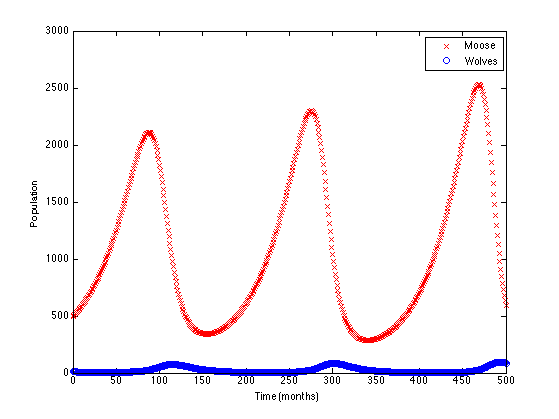
\includegraphics[width=4in]{figs/WolfMooseTImeSeries}
\caption{Simple Lotka-Volterra timeseries results for Wolf-Moose system with a timestep of one month.  $\beta = 0.025, \gamma = 0.057, W_c = 25, M_c=1000, M(1) = 500, W(1) = 10$.}
\end{figure}

This is a pretty awful graph -- you can't see what the wolf population is; the fonts are horrible; the font size is almost illegible -- but as a first output from our modeling effort, it's not bad.  

It appears that both populations are oscillating (which we expect).  On the other hand, it looks like the magnitude of the oscillations is growing -- is that something that makes physical sense, or is that an artifact of the model?

Let's dig into this a little more.  For now, we'll plot wolves and moose on separate axes:

\begin{verbatim}
figure;
subplot(2,1,1) % Create 2 stacked plots; plot in first of them
plot(T,M,'rx');
ylabel('Moose','FontSize',16)
subplot(2,1,2) % Now plot in the second set of axes
plot(T,W,'bo');
ylabel('Wolves','FontSize',16)
xlabel('Time','FontSize',16)
\end{verbatim}

Which gives us (the still not super-professional looking) plot: 

\begin{figure}[h!]
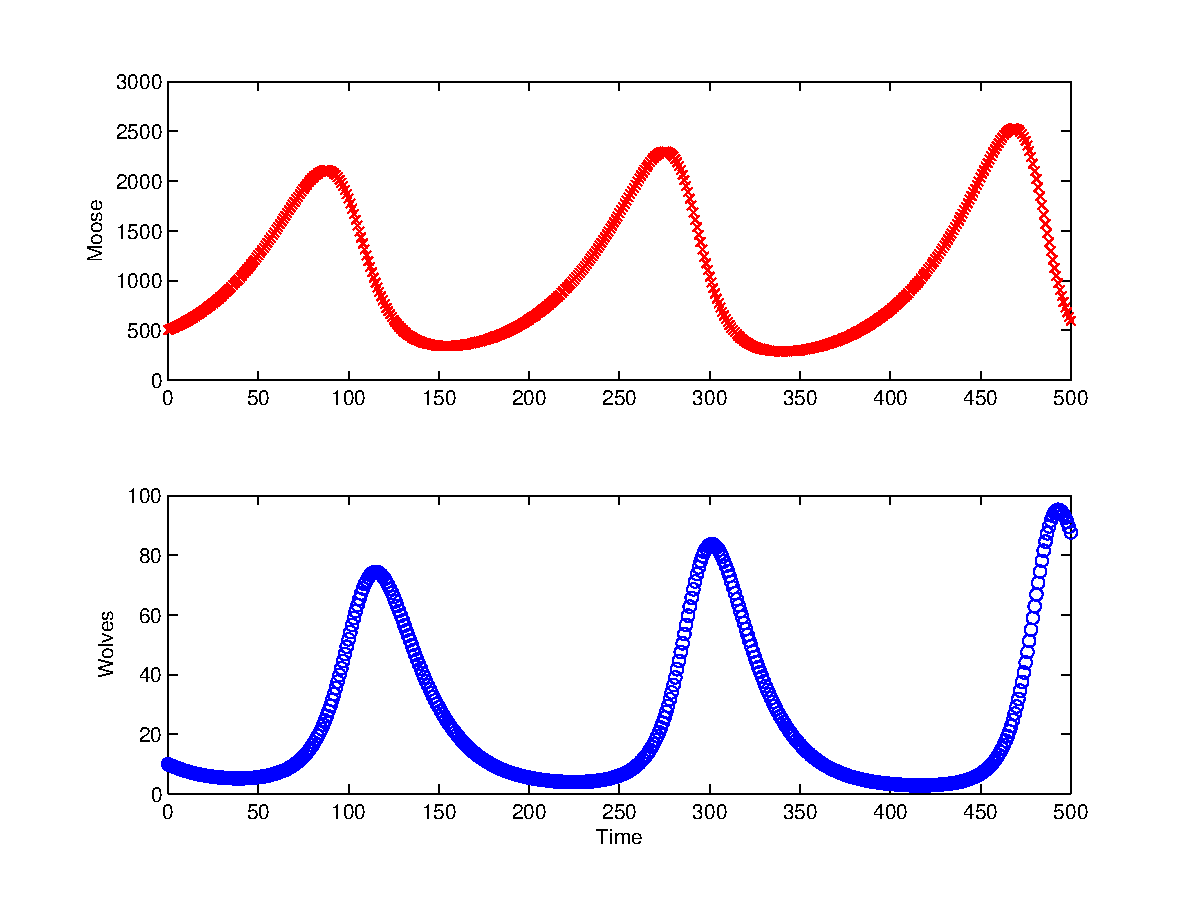
\includegraphics[width=4.5in]{figs/StackedWolfMooseTimeSeries}
\caption{Improved plot of Lotka-Volterra timeseries results for Wolf-Moose system with a timestep of one month.  $\beta = 0.025, \gamma = 0.057, W_c = 25, M_c=1000, M(1) = 500, W(1) = 10$.}
\end{figure}

Another option would be to examine the same data with a different visualization approach.  Let's plot $W$ versus $M$ -- i.e., the phase plane:

\begin{verbatim}
figure;
plot(M,W);
xlabel('Moose')
ylabel('Wolves')
\end{verbatim}

\begin{figure}[h!]
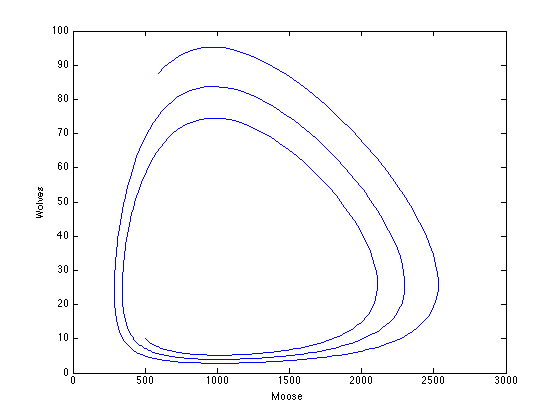
\includegraphics[width=4in]{figs/WolfMooseMATLABPP}
\caption{MATLAB Phase plane for Wolf-Moose system with a timestep of one month.  $\beta = 0.025, \gamma = 0.057, W_c = 25, M_c=1000, M(1) = 500, W(1) = 10$.}
\end{figure}


OK, what can we see here?  Well, the growing magnitude of the oscillation appears to be present in both the wolf and the moose populations.  It also looks like the actual wolf population gets AWFULLY small...  I wonder what will happen if we run for a longer time...

\begin{verbatim}
[M,W,T] = IRSimpleTimeSeries(500,10,.025, .057, 1000, 25,3000)
\end{verbatim}

\begin{figure}[h!]
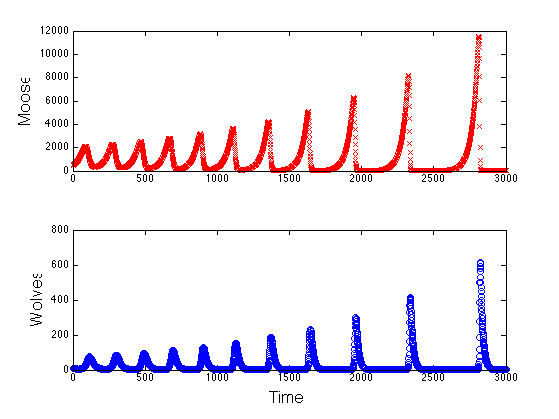
\includegraphics[width=4in]{figs/StackedWolfMooseTimeSeriesLongTime}
\caption{Lotka-Volterra timeseries results for Wolf-Moose system with a timestep of one month, runtime of 3000 months.  $\beta = 0.025, \gamma = 0.057, W_c = 25, M_c=1000, M(1) = 500, W(1) = 10$.}
\end{figure}

Hmm... This is not looking super physical - the peak populations seem to be going up, and up, and up; and the minimum populations seem to be getting really small.  If I poke at the actual numbers a little bit close to the end of the time series, I find some disconcerting results:

\begin{verbatim}
>> M(2400)
ans =
    0.5533
    
>> W(2500)
ans =
    0.0342
    
\end{verbatim}
Half a moose and $3\%$ of a wolf???  That doesn't make sense!  Does it?
 
\newthought{At this point we might want to take a deep breath,} look back at what we did, and think about ways to interpret it.  
 
 On one hand, we just ran a simulation of the wolf and moose populations for {\it 250 years}.  Do we really {\it expect} this model to tell us something  about 250 years of wolf and moose populations?  That seems suspect.

Furthermore, the qualitative physical behavior of the model is actually not too dissimilar from the behavior of the actual data.  Let's look back at the data for a second:

\beforefig
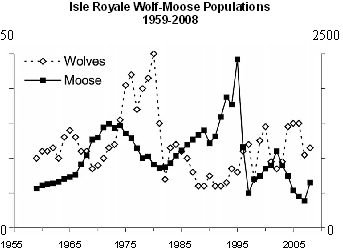
\includegraphics[width=4.5in]{figs/wolfmoosedata.jpg}


\afterfig

If we focus on the first twenty years of data, and squint a bit, you can see a similar rise and fall in moose population, followed by a rise and fall of the wolf population -- qualitatively similar to what we see in the model. The timescale is not exactly the same -- but it's {\it well} within a factor of 2, which is a reasonable starting point.

On the other hand, the growing amplitude behavior of the model (which is amplified at longer time periods) is a little disconcerting.   The long-term behavior is clearly non-physical, but doesn't that mean we should also be suspicious of the short-term behavior?

\section{Where do we go from here?}

At this point we could go in a number of directions.  One thing that might make sense would be to go back and re-examine the parameters.  We had relatively little confidence about our choices of $\beta$, $W_c$, $M_c$,  and particularly $\gamma$; we might want to use the existing data to try to determine better values of these parameters.  If we load the actual data into MATLAB and start down the dangerous road of tweaking parameters, it's not too hard to arrive at a reasonable {\it looking} result:

\begin{figure}[h!]
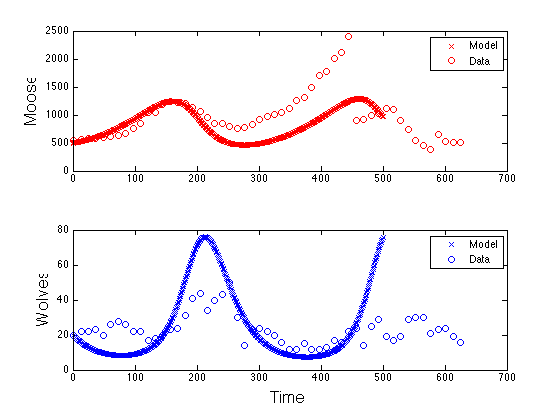
\includegraphics[width=4in]{figs/ModelDataComparison}
\caption{Comparison of model results and measured data  for Wolf-Moose system. Timestep of one month,  $\beta = 0.01, \gamma = 0.05, W_c = 30, M_c=800, M(1) = 500, W(1) = 20$.}
\end{figure}

However, if we poke at physical reality a bit, we learn that the drop in wolf population around month 280 was actually due to human introduction of a canine parvovirus -- so the nice match there is a little fishy.  Furthermore, to obtain this match, the parameter $\beta$ (which we were probably most confident about!) had to be reduced by more than 50\%.  If we look back at how we determined $\beta$, it was derived from the kill rate (moose per wolf per month).  The new kill rate this value of $\beta$ implies is about $2.6$ moose per wolf per month -- which is a {\it lot} higher than the measured data.  So some skepticism is warranted here -- I would NOT trust this model to tell me much about the future.

On the other hand, as we tweak parameters, we do learn about the impact these parameters have on the behavior of the model: changing, for example, $\beta$ effects behavior in interesting ways.  Similarly, 
we could investigate our choice of timestep.  We chose months for not particularly compelling reasons.  Does the model behavior change if we use days instead?  We would, of course, have to recompute our parameter values to make them appropriate for a different timestep!

Both of these options are in the space of testing the existing model.  But in some ways these investigations actually {\it could} form the basis for doing some work with the model.  For example, investigating the effect of changing $\beta$ is effectively asking the question, ``How does prey birthrate impact the qualitiative behavior of a simple predator-prey model?,'', or ``What kinds of qualitative changes might we expect on Isle Royale if we introduced a birth control plan for moose?''

At the same time our investigations have already illuminated an interesting issue:  for certain initial populations, you will hit a very low moose and/or wolf population at some point in the relatively near future (due to the oscillating behavior of the system).  Particularly for the wolves, such a situation places their survival at risk due to genetic issues as well as good old random chance.  You could ask the question, ``What initial populations avoid putting wolves at risk over a given time window?''.  Or you could improve your model to include probabilities in the low population condition; then you could do some kind of assessment of how the probability of species survival depended on initial populations.

And finally, you could decide that while this model is interesting, it doesn't answer the question you're interested in, and therefore needs to be taken back to the abstraction stage, so that you can add additional model terms that capture the effect you are interested in (e.g., a stock of ticks, or a stock of balsams, or an exogenous variable for weather patterns).  

\section{Doing Work}

Thus far we've created a very simple model for the population dynamics of wolves and moose on Isle Royale.  The model appears to have dynamics that are qualitatively similar to, but certainly not the same as, the observed dynamics in the physical system; and the parameters in the model, while not entirely grounded in measurements from the system, are at least reasonable in an order-of-magnitude sense.  

As outlined above, we could head in any number of directions at this point.  For the purposes of showing some examples of doing work, we'll look at a simple one: exploring the impact of moose population control.
This topic seems reasonable as a direction for work with this model.  First, it  involves something that {\it the model can tell us} -- as opposed to questions that trivially reflect something {\it we tell the model}.  Second, it doesn't involve making huge initial changes to the model.  Finally, it actually might matter in some real situation.  While we might not {\it really} want give the isle royale moose birth control pills, there are plenty of situations in which there is a desire to control a prey species population (think about deer in suburbs), so the learning we find from the investigation of moose population control might give us insights to other situations.  .

\subsection{Initial experiments with birth control}

How would our model change if we introduced some form of moose birth control?  The simplest way to model this would be simply to change the value of $\beta$ in our model:  $\beta$ represents the moose reproduction rate in the absence of wolves; if we start administering some form of birth control, presumably there will be fewer moose calves born per moose per year -- i.e., $\beta$ will be smaller.

If we look back at how we determined the parameters of the model, we figured out $\beta$ by looking at the moose kill rate, and at the critical densities of wolves and moose ($W_c$ and $M_c$).  $\beta$ was determined from these parameters.  Recalling the meaning of these parameters, $W_c$ is the number of wolves necessary to just offset moose reproduction.  If we start giving the moose birth control, presumably $W_c$ must be smaller -- which will in turn lead to $\beta$ being smaller.  On the other hand, the kill rate and the critical moose population both will presumably stay the same.

We'll take these ideas into account, and run two simulations:  one with the original value of $W_c$ and $\beta$, and one with slightly reduced values of these:

\begin{verbatim}
% Original values of parameters
gamma = 0.05
W_c = 30
M_c = 800
M_0 = 500
W_0 = 20
K=1
beta = K*W_c/M_c;

%Modified values of parameters
W_c2=W_c*0.9
beta2=K*W_c2/M_c;

%Calculate moose and wolf populations for both original and modified
[M,W,T] = IRSimpleTimeSeries(M_0,W_0,beta, gamma, M_c,W_c,500)
[M2,W2,T2] = IRSimpleTimeSeries(M_0,W_0,beta2, gamma, M_c,W_c2,500)
\end{verbatim}

Plotting both the original and the new timeseries, we see two interesting behaviors: first, the period of the oscillation for both populations seems to be longer.  Second, the amplitude of the oscillation for both populations is reduced.
\begin{figure}[h!]
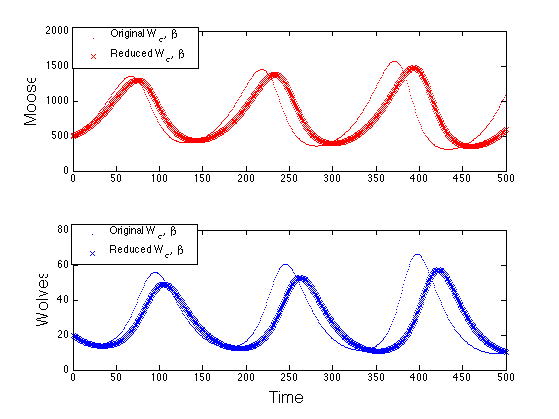
\includegraphics[width=4in]{figs/MooseBCTimeSeries}
\caption{Comparison of model results for different values of  $W_c$ and correspondingly changed 
$\beta$.  Timestep of one month,  $\gamma = 0.05, M_c = 800, K=1$, original $W_c = 30$; reduced
$W_c = 27$.}
\end{figure}

\subsection{Defining figures of merit}

Now, two data points does not make a trend, but it does cause us to wonder whether there is some kind of general behavior here.  How would we investigate this behavior?  We'd probably want to define a couple of {\em figures of merit} for the simulation:  numbers that characterize the overall behavior of a given timeseries.  In this case, the figures of merit are pretty obvious:  {\em period of oscillation} (let's call it $T$), and {\em amplitude of oscillation} (call it $A$).  By finding these two numbers for a given simulation, we have a short-hand way of talking about what the behavior of the simulation is.


If you've a skeptical type, you'd be well justified in throwing up your hands here and saying, ``Hold on just a minute here!  The period of oscillation and the amplitude of oscillation are both changing in time!  We saw that above when we went to long timescales!''  And you would be right:  strictly speaking, neither amplitude nor period are well-defined figures of merit for these timeseries.  But perhaps it's sensible to talk the initial amplitude and the initial period -- i.e., the distance between the first two peaks, and the distance between the first minimum and the first maximum.  These are at least well-defined.  Whether they are sensible remains to be seen.

Probably the easiest way to calculate these figures of merit is to determine where in time the minimums and maximums are in the vectors $M$ and $W$, and then use those locations to determine both the period and the amplitude.  Using the power of MATLAB (and I'll warn you that the code that follows is very MATLAB-ish):

\begin{verbatim}
function [TM,TW,AM,AW] = FindPeriodAndAmplitude(M,W,T)

    % vector that is zero if negative derivative, 1 if positive derivative
    DerivSignW=diff(W)>0; 

    %Find locations at which the sign of the derivative changes
    ZDW=find(diff(DerivSignW)~=0); 

    %Extract the first amplitude value
    AW=abs(W(ZDW(1))-W(ZDW(2))); 

    % Compute the period (min to min or max to max)
    TW = T(ZDW(3))-T(ZDW(1)); 

    %Same drill for Moose
    DerivSignM=diff(M)>0; 
    ZDM=find(diff(DerivSignM)~=0); 
    AM=abs(M(ZDM(1))-M(ZDM(2))); 
    TM = T(ZDM(3))-T(ZDM(1));

end
\end{verbatim}

\subsection{A parametric sweep and a punchline graph}

Once we've defined a figure of merit, it makes sense to use the figure of merit to investigate multiple scenarios.  One standard way to do this is with a {\it parameter sweep}:  we run the simulation over and over again for different values of a given parameter, and for This allows us to run some experiments like this, where we sweep $W_c$:

\begin{verbatim}
% Loop through different values of W_c,
% Find the timeseries for each
% Then extract the amplitudes, etc.
% Store them all
% And plot them


% Loop through different values of W_c

for i=1:50
    %Caluculate timeseries
    [M,W,T] = IRSimpleTimeSeries(M_0,W_0,beta, gamma, M_c,W_c,2000);
    % Make a plot
    hold on
    %Extract stuff
    [TM(i),TW(i),AM(i),AW(i)] = FindPeriodAndAmplitude(M,W,T);
    % Store current values of W_c and beta
    CritW(i) = W_c;
    B(i) = beta;
    W_c = W_c *0.995;
    beta = K*W_c/M_c;
end

figure;
subplot(2,1,1)
    
\end{verbatim}
and so on...

This gives us what might be referred to as the {\em punchline graph} for the question we asked:  we were interested in understanding how implementing moose birth control might change the dynamics of the system.  We investigated this by running a set of simulations for different levels of birth control.  We find, having done so, that at least for the initial conditions we're examining, the amplitude of oscillation decreases as we suppress moose reproduction, and the period of oscillation becomes longer.  \begin{figure}[h!]
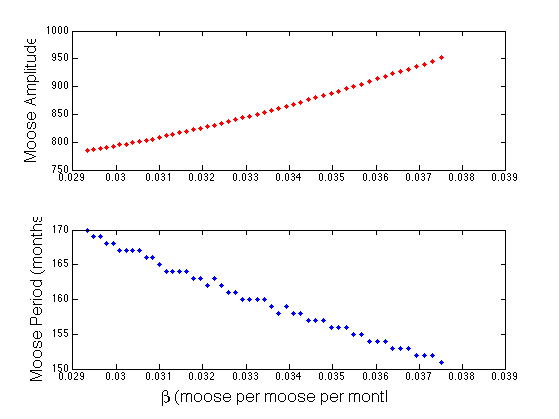
\includegraphics[width=4in]{figs/MooseBCSweepClean}
\caption{Amplitude and period of moose population for sweep of moose birth rate and critical wolf population $W_c$.  Timestep of one month,  $\gamma = 0.05, M_c = 800, K=1$.  Note that the period exhibits discrete steps due to the discrete time model}
\end{figure}

This figure makes the argument much more compellingly than does the comparison of two different time series.  Of course, we'd probably want to show the timeseries first -- both so that a reader can see what the behavior is, and so that the figures of merit we have defined are explained -- but as an answer to the question, this graph is much stronger.

\begin{del}

If you investigate further, you'll find some very surprising, and rather suspicious, behavior.  When you sweep down further in birthrate, initially the amplitude decreases, and the period increases -- all very consistent with our initial observation.  However, at around $\beta = 0.025$, there's a sharp discontinuity in the amplitude, and the value of the amplitude starts increasing instead of  decreasing.   This looks an awful lot like some kind of artifact.  What is going on here?  Does this invalidate our results above?

\begin{figure}[h!]
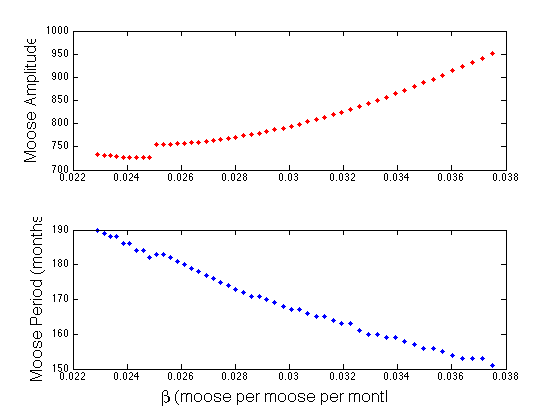
\includegraphics[width=4in]{figs/MooseBCSweep}
\caption{Amplitude and period of moose population for sweep of moose birth rate and critical wolf population $W_c$.  Timestep of one month,  $\gamma = 0.05, M_c = 800, K=1$.}
\end{figure}

\end{del}
